\documentclass[a4paper,12pt]{article}

% Se vuoi che il pdf sia in formato mobile, decommenta la linea qui sotto e commenta la prima linea del codice
%\documentclass[1pt]{article}
\usepackage{enumitem}
\usepackage[paper size={90mm, 160mm},left=2mm,right=2mm,top=2mm,bottom=2mm,nohead]{geometry}
\usepackage{microtype}
\setlist[itemize]{leftmargin=*}


\usepackage{float}
\usepackage{url}
\usepackage{xcolor}
\usepackage{pdfpages}
\usepackage{graphicx}


%Comando per creare nuove definizioni stile blocco
\newcommand{\definition}[2]{
	\begin{table}[H]
	\centering
		\begin{tabular}{|p{0.9\linewidth}}
		\textbf{#1}\\ %Titolo della definzione
		#2\\%Testo della definizione
		\end{tabular}
	\end{table}
	\noindent
}

\newcommand{\df}[2]{\definition{#1}{#2}}

%%%%%%%%%%%%%%%%%%%%%%%%%%%%%%%%%%%%%%%%%%%%%%%%%%%%%%%%%%%%%%%%%%%%%
%      INSBOX --- macros for inserting pictures into paragraphs     %
%       Micha\l{} Gulczy\'nski, Szczecin, Jan 1996 / Feb 1998       %
%                     mgulcz@we.tuniv.szczecin.pl                   %
%%%%%%%%%%%%%%%%%%%%%%%%%%%%%%%%%%%%%%%%%%%%%%%%%%%%%%%%%%%%%%%%%%%%%
%
%  version 2.2
%
%  available macros:
%    * \InsertBoxC{anybox}
%        insert a centered box (use int _inside_ a paragraph)
%    * \InsertBoxL{after_line}{anybox}[correction]
%    * \InsertBoxR{after_line}{anybox}[correction]
%        insert a box in the left/right after specified number of lines;
%        correction specified in square brackets is optional;
%        both macros should be called _before_ a paragraph
%    * \MoveBelowBox
%        start a new paragraph just below the current frame
%
%  see the demo.tex file for more information
%

\catcode`\@ = 11
%
%  Margin between the text and the box:
\newdimen\@InsertBoxMargin
\@InsertBoxMargin = 2mm
%
%  definition of \ParShape, an inproved version of plain \parshape
%
\newcount\@numlines    % sum: m_1+...+m_n
\newcount\@linesleft   % counter used when reading lines of \ParShape
\def\ParShape{%
    \@numlines = 0
    \def\@parshapedata{ }% here we'll collect data for plain \parshape
    \afterassignment\@beginParShape
    \@linesleft
}%
\def\@beginParShape{%
    \ifnum \@linesleft = 0
      \let\@whatnext = \@endParShape
    \else
      \let\@whatnext = \@readnextline
    \fi
    \@whatnext
}%
\def\@endParShape{%
    \global\parshape = \@numlines \@parshapedata
}%
\def\@readnextline#1 #2 #3 {% #1 #2 #3 are: m_i, leftskip_i, rightskip_i
    \ifnum #1 > 0
      \bgroup  % I want to keep changes of \dimen0 and \count0 local
        \dimen0 = \hsize
        \advance \dimen0 by -#2  % \parshape requires left skip and
        \advance \dimen0 by -#3  % _length_of_line_ (not right skip!)
        \count0 = 0
        \loop
          \global\edef\@parshapedata{%
            \@parshapedata    % add to \@parshapedata:
            #2                % left skip
            \space            % a space
            \the\dimen0       % length of line
            \space            % another space
          }%
          \advance \count0 by 1
          \ifnum \count0 < #1
        \repeat
      \egroup
      \advance \@numlines by #1
    \fi
    \advance \@linesleft by -1
    \@beginParShape
}%
%
%  \InsertBoxC, \InsertBoxL, \InsertBoxR
%
\newbox\@boxcontent     % box containing the picture to be inserted
\newcount\@numnormal    % number of leading lines to typeset normally
\newdimen\@framewidth   % width of the frame
\newdimen\@wherebottom  % position of frame's bottom
\newif\if@byframe       % true if we are just beside the frame
\@byframefalse
%
%
\def\InsertBoxC#1{%
  \leavevmode
  \vadjust{
    \vskip \@InsertBoxMargin
    \hbox to \hsize{\hss#1\hss}
    \vskip \@InsertBoxMargin
  }%
}%
\def\InsertBoxL#1#2{%
  \@numnormal = #1
  \setbox\@boxcontent = \hbox{#2}%
  \let\@side = 0
  \futurelet \@optionalparameter \@InsertBox
}
\def\InsertBoxR#1#2{%
  \@numnormal = #1
  \setbox\@boxcontent = \hbox{#2}%
  \let\@side = 1
  \futurelet \@optionalparameter \@InsertBox
}%
\def\@InsertBox{%
  \ifx \@optionalparameter [
    \let\@whatnext = \@@InsertBoxCorrection
  \else
    \let\@whatnext = \@@InsertBoxNoCorrection
  \fi
  \@whatnext
}%
\def\@@InsertBoxCorrection[#1]{%
  \ifx \@side 0
    \@@InsertBox{#1}{0}{{\the\@framewidth} 0cm}%
  \else
    \@@InsertBox{#1}{1}{0cm {\the\@framewidth}}%
  \fi
}%
\def\@@InsertBoxNoCorrection{%
  \@@InsertBoxCorrection[0]%
}%
\def\@@InsertBox#1#2#3{%
  \MoveBelowBox
  \@byframetrue
  % \@wherebottom = \pagetotal + (\@numnormal * \baselineskip) +
  %                 (height of \@boxcontent) + (2 * \@InsertBoxMargin)
  \@wherebottom = \baselineskip
  \multiply \@wherebottom by \@numnormal
  \advance \@wherebottom by 2\@InsertBoxMargin
  \advance \@wherebottom by \ht\@boxcontent
  \advance \@wherebottom by \pagetotal
  % I have no idea why, but \InsertBox called at the top of a page
  % calculates space for the box one line too big
  \ifdim \pagetotal = 0cm
    \advance \@wherebottom by -\baselineskip  % ^ reduction
  \fi
  % add the correction
  \advance \@wherebottom by #1\baselineskip
  % \@framewidth = (width of \@boxcontent} + \@InsertboxMargin
  \@framewidth = \wd\@boxcontent
  \advance \@framewidth by \@InsertBoxMargin
  %
  \bgroup  % to keep changes of \dimen0 local
    % check if the box fits in the page
    \ifdim \pagetotal = 0cm
      \dimen0 = \vsize
    \else
      \dimen0 = \pagegoal
    \fi
    \ifdim \@wherebottom > \dimen0
      % print a warning message ...
      \immediate\write16{+--------------------------------------------------------------+}%
      \immediate\write16{| The box will not fit in the page. Please, re-edit your text. |}%
      \immediate\write16{+--------------------------------------------------------------+}%
      % ... and mark this place in document with a black box
      \vrule width \overfullrule
    \fi
  \egroup
  \prevgraf = 0
  % insert the box in the left (if #2 = 0) or in the right (if #2 = 1)
  \vbox to 0cm{%
    \dimen0 = \baselineskip
    \multiply \dimen0 by \@numnormal
    \advance \dimen0 by -\baselineskip
    \setbox0 = \hbox{y}%
    \vskip \dp0
    \vskip \dimen0
    \vskip \@InsertBoxMargin
    \ifnum #2 = 1
      \vtop{\noindent \hbox to \hsize{\hss \box\@boxcontent}}%
    \else
      \vtop{\noindent \box\@boxcontent}%
    \fi
    \vss
  }%
  % I have no idea why, but this is really necessary
  \vglue -\parskip
  \vskip -\baselineskip
  % each following paragraph needs to be formatted properly
  \everypar = {%
    % are we already below the bottom of the box?
    \ifdim \pagetotal < \@wherebottom
      % no...
      \bgroup  % to keep some changes local
        % let's calculate parameters for \ParShape
        \dimen0 = \@wherebottom
        \advance \dimen0 by -\pagetotal
        \divide \dimen0 by \baselineskip
        \count1 = \dimen0
        \advance \count1 by 1
        \advance \count1 by -\@numnormal
        \ifnum #2 = 1
          \ParShape = 3
                      {\the\@numnormal}   0cm   0cm
                      {\the\count1}       0cm   {\the\@framewidth}
                      1                   0cm   0cm
        \else
          \ParShape = 3
                      {\the\@numnormal}   0cm                  0cm
                      {\the\count1}       {\the\@framewidth}   0cm
                      1                   0cm                  0cm
        \fi
      \egroup
    \else
      % yes!
      \@restore@    % it's time to end everything
    \fi
  }%
  % this definition isn't very necessary --- just in case the paragraph
  % following \InsertBoxL or \InsertBoxR has fewer lines that the
  % first argument of the macro
  \def\par{%
      \endgraf
      \global\advance \@numnormal by -\prevgraf
      \ifnum \@numnormal < 0
        \global\@numnormal = 0
      \fi
      \prevgraf = 0
  }%
}%
%
%  call this macro to move the current position just below the
%  current frame
%
\def\MoveBelowBox{%
  \par
  \if@byframe
    \global\advance \@wherebottom by -\pagetotal
    \ifdim \@wherebottom > 0cm
      \vskip \@wherebottom
    \fi
    \@restore@
  \fi
}%
%
%  normal settings are as follows:
%
\def\@restore@{%
    \global\@wherebottom = 0cm
    \global\@byframefalse
    \global\everypar = {}%
    \global\let \par = \endgraf
    \global\parshape = 1 0cm \hsize
}%
%
%  someone told me that in LaTeX there is no \pageno counter;
%  the counterpart is \c@page
%
\ifx \documentclass \@Dont@Know@What@It@Is@
\else
  \let \pageno = \c@page
\fi


\catcode`\@ = 12

\newcommand{\lessonDate}[1]{\InsertBoxR{0}{\tiny{#1}}}

\newcommand{\E}{\`E\space}

\usepackage{listings}
\lstset{language=C++,
                keywordstyle=\color{blue},
                stringstyle=\color{red},
                commentstyle=\color{green},
                morecomment=[l][\color{magenta}]{\#}
}

\sloppy
\begin{document}

\begin{titlepage}
\begin{center}
	\Large{\textbf{Appunti di Sicurezza Informatica}}
\vfill
\normalsize{Caccaro Sebastiano}\\
\normalsize{A.A.2019/2020}
\end{center}
\end{titlepage}

\tableofcontents

\clearpage


%Lezione di 10 Ottobre 2019
\lessonDate{10 Ottobre 2019}
\section{Introduzione}
\textbf{Sito del corso}: \url{http://security.di.unimi.it/sicurezza1920/sec2.shtmls}\\
L'esame sarà a febbraio\\
\textbf{Modalità esame}: parte a quiz fatta computer + parte pratica sempre fatta a computer.

\section{Memory Errors}
Specialmente in certi linguaggi di programmazione, come C e C++, che non hanno meccanismi di controllo su quello che fa il programmatore con la memoria. Posso quindi sovrascrivere zone di memoria che non sono di mia competenza. Posso quindi creare degli \textbf{unexpected behaviour}.\\
Posso usare queste falle per comportamenti malevoli, come eseguire codice scritto da un attaccante ecc, per rubare dati ecc.\\
Sono scritti in C o C++ componenti che devono essere velocissimi, come sistemi operativi e sistemi critici, server web, embedded sistems.\\
Altri linguaggi non hanno questi problemi perchè inseriscono dei controlli, ma a scapito delle perfomance.

\subsection{Buffer Overflow}
\subsubsection{Storia}
Comincia del 1988 con il \textbf{Morris Worm}. Nel giro di 3-4 ore butta giù tutta la DarpaNet, prendendo una multa di 10-100 milioni di dollari, galera ecc.
\definition{Worm}{Programma che si autoreplica e si diffonde in varie macchine}
Nel 2001 \textbf{Code Red} infetta 300.000 macchine in 14 ore, nel 2003 \textbf{SQL Slammer} infetta 75.000 macchine in 10 minuti.\\
Molte vulnerabilità non vengono mai corrette, perchè comunque l'applicazione funziona lo stesso.
\subsubsection{Layout di memoria}
\definition{Memoria Virtuale}{Modalità di visualizzazione della memoria nella quale un processo vede tutta la memoria come se fosse assegnata solo a lui.}

\begin{figure}[H]
	\centering
	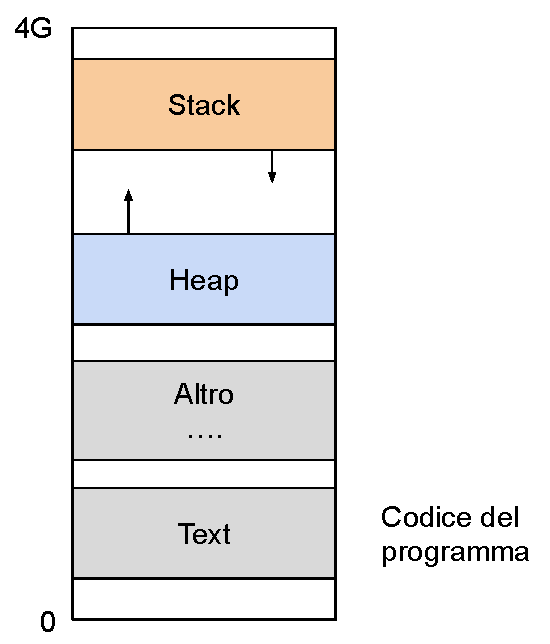
\includegraphics[width=0.5\linewidth]{Immagini/Stack1.pdf}
	\caption{Layout di memoria nei processori Intel}
\end{figure}

Mentre lo Stack cresce verso il basso, lo Heap cresce verso l'alto. Quindi, se nello stack per allocare devo sottrarre (andare giu), nello heap devo andare verso l'alto.\\
Lo Heap contiene perlopiù variabili allocate dal programmatore. Nello Heap, per allocare memoria, devo usare \texttt{malloc(sizeof(tipo))}. Una volta che non mi serve più quella zona, la libero con un \texttt{free}.

\subsubsection{Funzionamento dello Stack}

\begin{figure}[H]
	\centering
	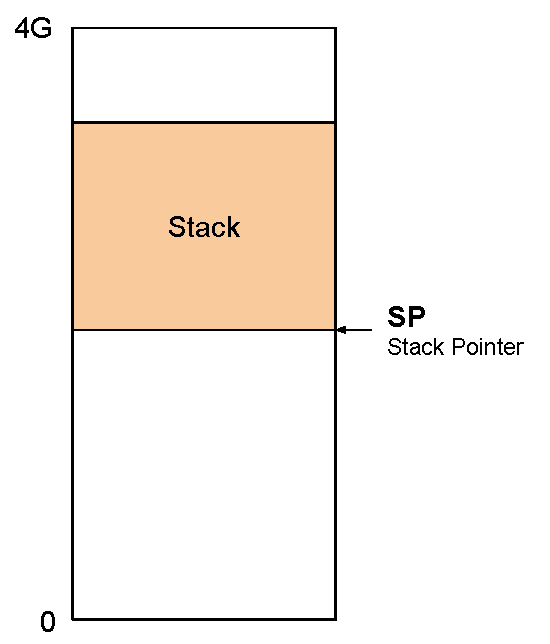
\includegraphics[width=0.5\linewidth]{Immagini/Stack2.pdf}
	\caption{Stack Pointer}
\end{figure}

Solitamente lo stack è utilizzato dal programma, in genere per le chiamate a funzioni. Lo stack è delimitato dallo \textbf{stack pointer}.

\begin{figure}[H]
\centering
\begin{lstlisting}[xleftmargin=.35\textwidth]
function(a1,b,c)
  int z
  strcpy(a,a1)
  return
  
main(...)
  function(a,b,c)
  Y:RET	
	
\end{lstlisting}
\caption{Esempio di chiamata a funzione}
\end{figure}

\begin{figure}[H]
	\centering
	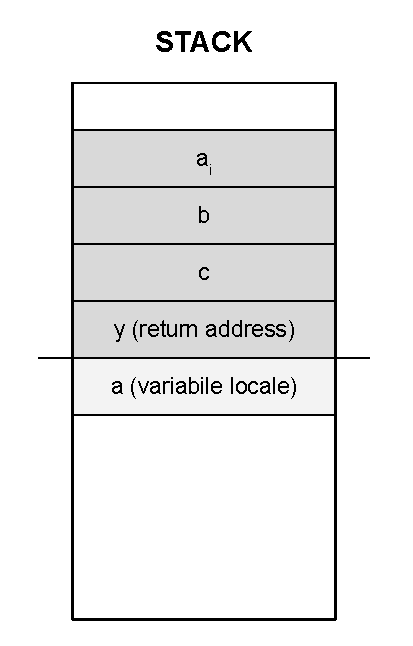
\includegraphics[width=0.4\linewidth]{Immagini/Stack3.pdf}
	\caption{Stack Pointer dell'esempio precedente}
\end{figure}

Quando vado ad eseguire la funzione, alloco anche un return address, che mi serve per capire dove andare alla fine della funzione. I parametri della funzione vengono poi espressi in funzione della posizione dello stack pointer (SP+16 bit ecc). Alla fine della funzione, sposto l'instruction a pointer viene impostato con il valore presente in Y, ovvero il return address. \E compito del chiamante poi togliere dallo stack gli altri parametri (\texttt{a}, \texttt{b} e \texttt{c}).
Cosa succede quindi ad una chiamata?\\
Chiamando la funzione:
\begin{enumerate}
\item Push degli argomenti nello stack
\item Push del return address
\item Jump all'indirizzo della funzione
\end{enumerate}
Tornando alla funzione principale:
\begin{enumerate}
\item Ritorno allo stack frame precedente
\item Torno al return address
\end{enumerate}

\subsubsection{Problematiche}
\definition{Buffer Overflow}{Operazione di scrittura che va a eccedere la locazione di memoria allocata a un dato dato.}

\begin{figure}[H]
\begin{lstlisting}[language=C++, xleftmargin=.3\textwidth]
void func(char *arg1)
{
 int authenticated = 0;
 char buffer[4];
 strcpy(buffer, arg1);
 if (authenticated) {...
 ...
}

int main()
{
 char *mystr = "AuthMe!";
 func(mystr);
 ...
}
\end{lstlisting}
\caption{Programma che esegue un buffer overflow}
\end{figure}

\begin{figure}[H]
	\centering
	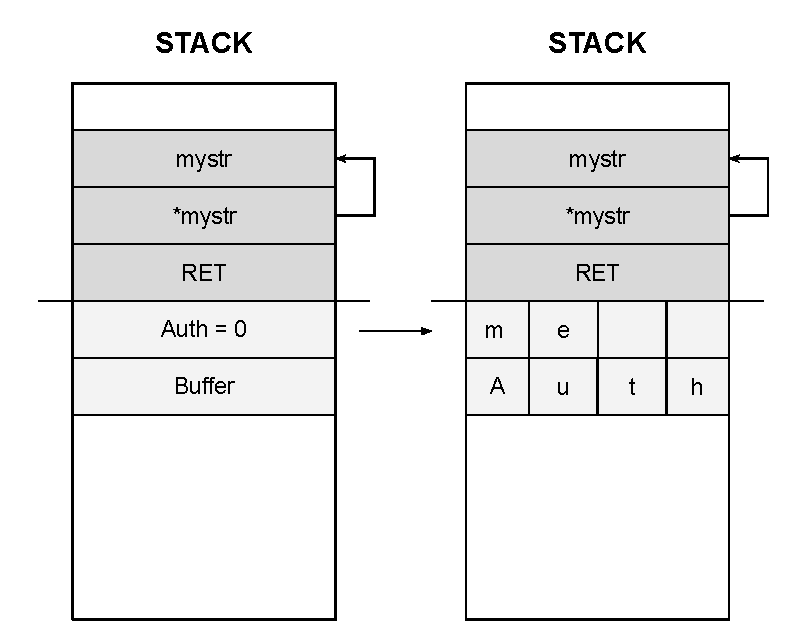
\includegraphics[width=0.8\linewidth]{Immagini/Stack4.pdf}
	\caption{Stack dell'esempio precedente}
\end{figure}
Sto provando a copiare una stringa "\texttt{AuthMe}" nel buffer a 4 byte. Siccome un carattere corrisponde a un byte, riesco a copiare solamente "\texttt{Auth}". Quindi, per scrivere il "\texttt{Me}" devo andare sopra nello stack. Quindi ho scritto "\texttt{Me}" nella variabile \texttt{Authenticated}, che adesso è diversa da 0. Ora quindi sono autenticato!\\
Con questo metodod potrei tranquillamente sovrascrivere tutto lo stack. Potrei, ad esempio, \textbf{sovrascrivere il return address}, saltando quindi in qualsiasi punto all'interno del programma, addirittura a parti del codice inserite in modo malevolo.

\subsubsection{Code Injection}
Lo scopo di una \textbf{Code Injection} è quello di fornire il codice da eseguire all'interno del programma. Purtroppo non posso metterla all'interno della sezione \texttt{Text}, perchè è read-only. Mettiamo quindi il codice all'interno dello stack.

\begin{figure}[H]
\begin{lstlisting}[language=C++, , xleftmargin=.3\textwidth]
void func(char *arg1)
{
 char buffer[4];
 sprintf(buffer, arg1)
}
\end{lstlisting}
\caption{Snippet}
\end{figure}
L'idea è quella di sovrascrivere buffer fino al return address. Il mio scopo è quello di inserire il mio codice all'interno di buffer, fino ad arrivare alla zona di memoria del return address. Nel return address andrò quindi a puntare l'indirizzo di memoria nel buffer, andando quindi ad eseguire il codice contento all'interno di essa.\\
Ma come faccio a sapere l'indirizzo di memoria attuale del buffer? Siccome la memoria è virtuale, riesco a sapere più o meno un range dove si trova l'indirizzo del buffer. Quindi inserisco prima del codice una sequenza di \textbf{\texttt{NOP}}, una cosidetta \textbf{NOP-sled} (pista d'atterraggio) per il mio codice.
\definition{NOP}{Short for NO Operation. Istruzione assembly che dice al processore di non fare niente per un ciclo di clock}

Devo quindi avere le seguenti cose:
\begin{itemize}
\item Distanza da sovrascrivere
\item Codice da inserire (inteso come codice macchina, binario, ancora più basso dell'assembly)
\item Indirzzo del buffer
\end{itemize}

Creo quindi il cosidetto \textbf{attack vector}.

\definition{Attack Vector}{Input che devo fornire al programma per inserire il mio exploit}

Per capire un po'meglio dove è il return address, provo a sovrascrivere con dati a caso sempre più grandi. Se il programma crasha, vuol dire che sta probabilmente cercando di saltare a un indirizzo a caso. Quindi è probabile che abbia trovato il return address.

\begin{figure}[H]
	\centering
	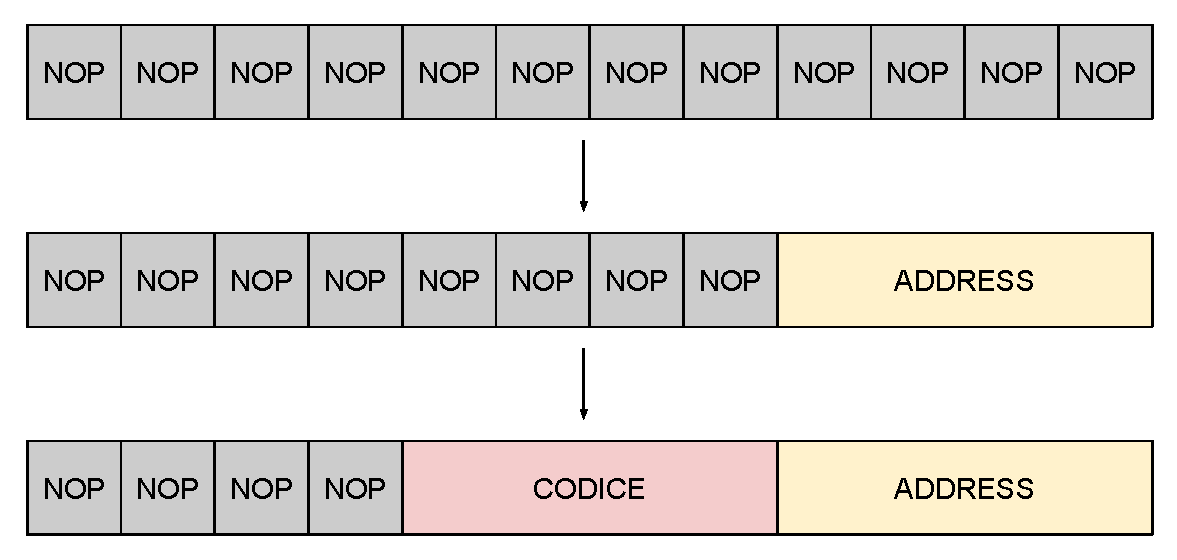
\includegraphics[width=0.8\linewidth]{Immagini/AttackV1.pdf}
	\caption{Costruzione di un attack vector}
\end{figure}

\begin{figure}[H]
	\centering
	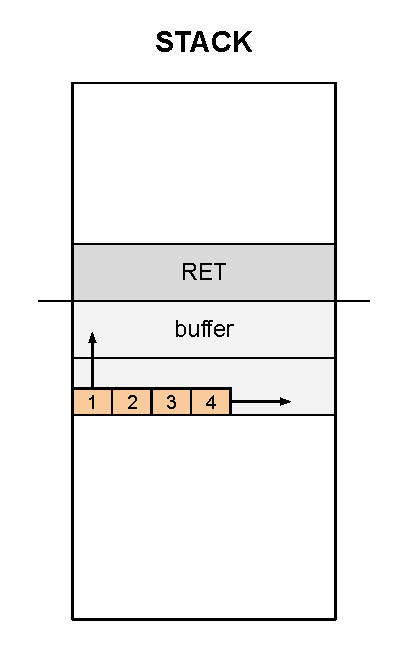
\includegraphics[width=0.4\linewidth]{Immagini/Stack5.pdf}
	\caption{Processo di scrittura della memoria}
\end{figure}
Il mio scopo solitamente è quello di acquisire maggiori privilegi. Lo faccio tramite qui programmi denominati \textbf{set whith rooot}, ovvero quei programmi che possono essere eseguiti da un utente normale ma che girano con permessi di root.

\subsubsection{Esempio di Code Injection}
Esercizio 1 disponibile qui \url{⎄https://github.com/andrealan/Software-Security-Lab/tree/master/bof-exercise}
\definition{Shell Code}{Codice che esegue una nuova finestra della shellS}
Il programma attaccante dichiara lo \textbf{shell code}. Nel main viene creato l'attack vector.
\begin{enumerate}
\item Creo un buffer
\item Lo riempio di NOP
\item Dichiaro l'offset rispetto al stack pointer, potrei doverlo cambiare
\item Inserisco il valore dell'indirizzo all'inizio
\item Scrivo lo shellcode dopo l'indirizzo
\end{enumerate}

\noindent\textbf{\Large IMPORTANTE}\\
 \textbf{La lettura nello stack avviene verso l'alto}. Quindi la NOP sled più che come una discesa, può essere pensata come un uno skilift.
 
\begin{figure}[H]
	\centering
	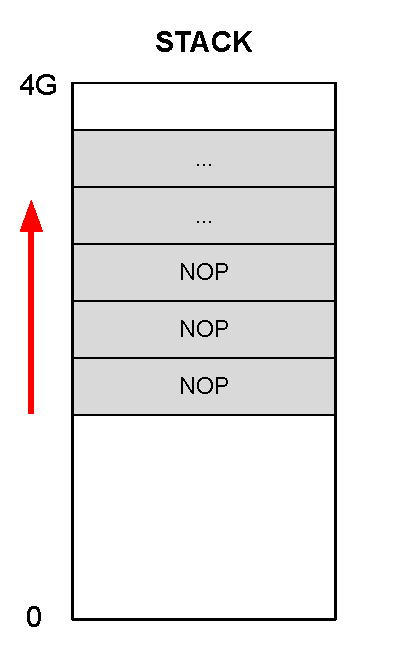
\includegraphics[width=0.4\linewidth]{Immagini/Stack6.pdf}
	\caption{La lettura dello stack avviene verso l'alto}
\end{figure}

\lessonDate{22 Ottobre}
\subsection{Heap Overflow}
\subsection{Concetti generali sull'allocazione nello Heap}
L'allocazione nello Heap è gestita manualmente dallo sviluppatore e consente l'allocazione di grosse strutture dati anche dinamicamente a run time. Generalmente è più lenta rispetto allo stack.\\
Le due operazioni permesse sullo Heap sono:
\begin{itemize}
\item \texttt{malloc(bytes)}: richiede l'allocazione di tot byte nello Heap.
\item \texttt{free(puntatore)}: libera una porzione di memoria precedentemente occupata.
\end{itemize}

\subsubsection{Heap Chunck}
Lo Heap è organizzato in \textbf{chunck}, struttura dati rappresentata in seguito.
\begin{figure}[H]
\begin{lstlisting}
struct malloc_chunk {
  /* Size of previous chunk (if free).  */
  INTERNAL_SIZE_T      prev_size;  
  /* Size in bytes, including overhead. */
  INTERNAL_SIZE_T      size;       

  /* double links -- used only if free. */
  struct malloc_chunk* fd;         
  struct malloc_chunk* bk;

/*Only used for large blocks: pointer to next larger size.*/
/*double links -- used only if free. */
  struct malloc_chunk* fd_nextsize; 
  struct malloc_chunk* bk_nextsize;
}
\end{lstlisting}
\end{figure}

\noindent\textbf{fd} e \textbf{bk} stanno per \textbf{forward} e \textbf{backwards}. Nello Heap, i blocchi liberi sono organizzati in liste doppiamente linkate con chunk di dimensioni simili. I blocchi occupati, non hanno tali puntatori.\\
Per ogni chunk, se il chunk precedente è libero, il bit meno significativo di INTERNAL\_SIZE\_T è posto a 0, altrimenti va posto a 1.

\begin{figure}[H]
	\centering
	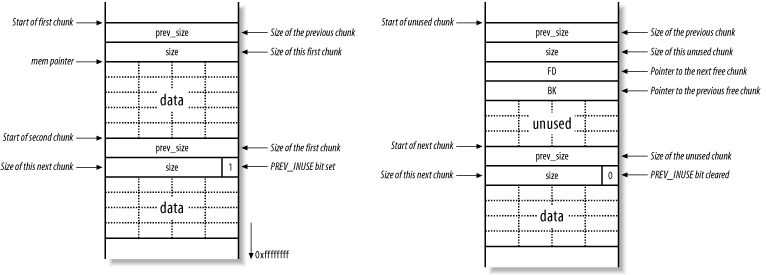
\includegraphics[width=\linewidth]{Immagini/Heap1}
	\caption{Sezione di Heap prima e dopo la free di un chunk}
\end{figure}
\subsubsection{Allocazione Memoria}
\noindent Il chunck che rappresenta la memoria libera nello Heap è detto \textbf{Top Chunk}. Ogni qualvolta voglio allocare nuova memoria, il top chunk viene diviso in due: una parte diventa memoria allocata, la parte rimasta libera diventa il nuovo top chunk.\\ Ovviamente si ricorre allo splitting del top chunck solamente se non ci sono chunk liberi di dimensioni idonee nelle liste di chunck liberi.

\begin{figure}[H]
	\centering
	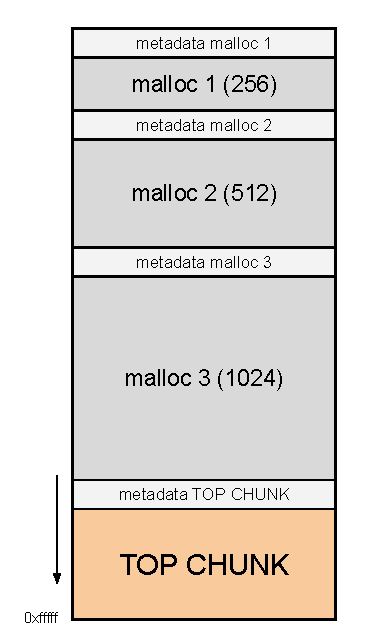
\includegraphics[width=0.4\linewidth]{Immagini/Heap2}
	\caption{Heap dopo un malloc di 256, uno di 512 e uno di 1024 in quest'ordine}
\end{figure}

\subsection{Deallocazione memoria}
Quando dealloco memoria svolgo le seguenti operazioni:
\begin{itemize}
\item Pongo a 0 il bit meno significativo del campo size del blocco successivo a quello che sto deallocando.
\item Pongo nel campo \texttt{prev\_size} del chunk successivo la dimensione del chunk che sto allocando.
\item In caso anche il chunk precedente sia libero, unisco i due chunk.
\end{itemize}
\subsubsection{Unsafe Unlink}
Quando vado a deallocare un chunck preceduto o succeduto da un un chunk libero, posso andare a mergiare questi due chunk.\\
Analizziamo il caso in cui il chunk precedente (p) a quello che devo deallocare sia libero. Svolgerò le seguenti operazioni:
\begin{itemize}
\item Incremento la size di p, inglobando il chunk successivo.
\item Eseguo l'\textbf{unlink} di p (che quindi ora ingloba anche il chunk che voglio deallocare)
\item Posiziono p nella lista di chunk più appropriata
\end{itemize}

\begin{figure}[H]
	\centering
	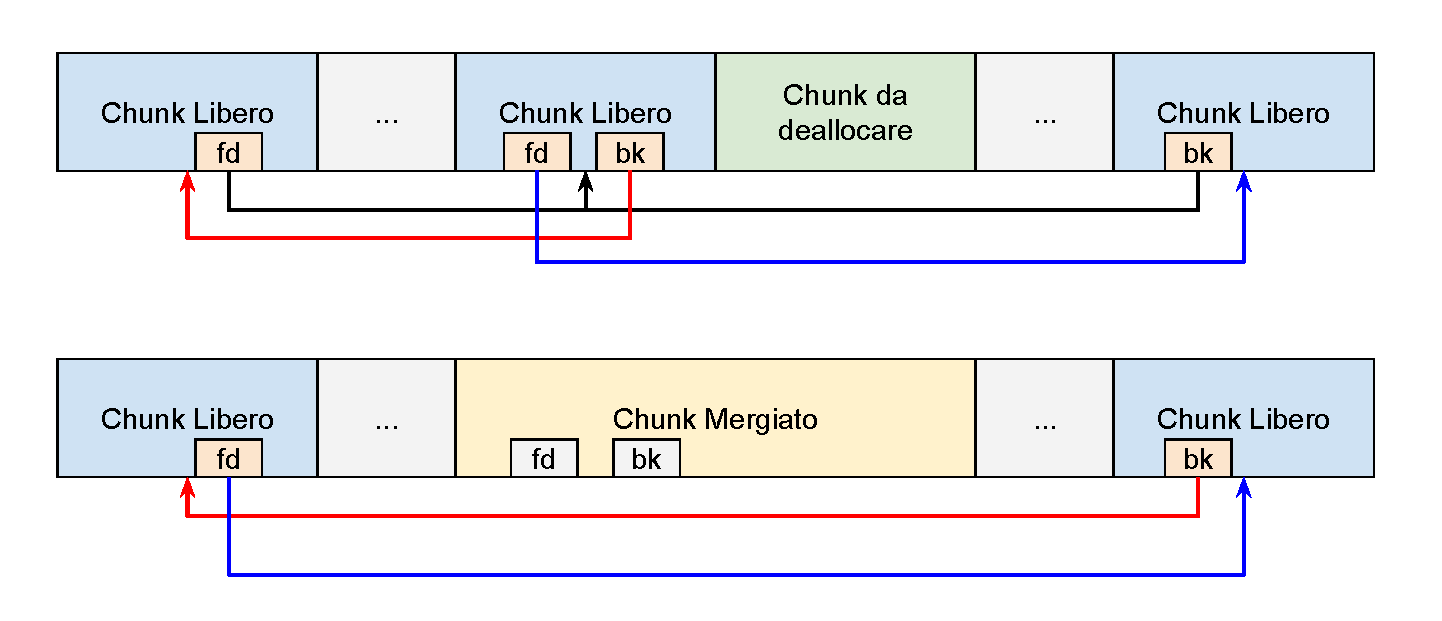
\includegraphics[width=\linewidth]{Immagini/Unlink}
	\caption{Situazione prima e dopo unlink}
\end{figure}

Questa procedura avviene tramite il seguente codice

\begin{figure}[H]
\begin{lstlisting}[language=C]
#define unlink(P, BK, FD) {
  FD = P->fd;
  BK = P->bk;
  FD->bk = BK;
  BK->fd = FD;
}
\end{lstlisting}
\end{figure}

http://etutorials.org/Networking/network+security+assessment/Chapter+13.+Application-Level+Risks/13.5+Heap+Overflows/

\lessonDate{24 Ottobre 2019}
\subsection{User After Free}
\E più legato a proprietà temporali della memoria che a proprietà spaziali. Rispetto ad altre vulnerabilità, è più difficile da individuare e da correggere. Ad oggi, è una delle vulnerabilità più usate e sfruttate. Ne sono state trovate in browser come Chrome, ma anche in altri browser.\\
In linguaggi come Java queste cose non sono possibili perchè sono presenti vari controlli sulla memoria. Rispetto a questa specifica vulnerabilità, Java si protegge tramite il garbage collector.\\
La user after free avviene quando una zona di memoria viene liberata, ma provo comunque a dereferenziare il puntatore che la puntava. Si basa quindi sui \textbf{dangling pointers}. Una volta deallocata una zona di memoria, è buona pratica settare il suo puntatore a 0.\\
Sostanzialmente, quello che si può fare è usare un dangling pointer per accedere a zone di memoria che dovrei lasciare stare.
\subsubsection{Esempio di Use After Free}
\begin{lstlisting}[language=C]
#include <stdlib.h>
#include <unistd.h>
#include <string.h>
#include <sys/types.h>
#include <stdio.h>

struct auth {
  char name[32];
  int auth;
};

struct auth *auth;
char *service;

int main(int argc, char **argv)
{
  char line[128];

  while(1) {
      printf("[ auth = %p, service = %p ]\n", auth, service);

      if(fgets(line, sizeof(line), stdin) == NULL) break;
      
      if(strncmp(line, "auth ", 5) == 0) {
          auth = malloc(sizeof(auth));
          memset(auth, 0, sizeof(auth));
          if(strlen(line + 5) < 31) {
              strcpy(auth->name, line + 5);
          }
      }
      if(strncmp(line, "reset", 5) == 0) {
          free(auth);
      }
      if(strncmp(line, "service", 6) == 0) {
          service = strdup(line + 7);
      }
      if(strncmp(line, "login", 5) == 0) {
          if(auth->auth) {
              printf("you have logged in already!\n");
          } else {
              printf("please enter your password\n");
          }
      }
  }
 }
\end{lstlisting}
Il programma è un loop continuo che chiede all'utente che servizi vuole. Posso scegliere fra 4 comandi, a seconda di quello che voglio fare. Il comando auth vuole una sintassi del tipo \texttt{auth admin}. Reset libera la memoria puntata da auth. Service copia la linea inserita e la mette dentro dentro \texttt{service}. Login controlla se io mi sono già loggato o no. Voglio autenticarmi anche se non so la password, mettendo auth$->$auth a 1. I passaggi per loggarsi sono i seguenti:
\begin{itemize}
\item Chiamo il comando \texttt{auth}, scrivendo tipo \texttt{auth seba}
\item Chiamo il reset, andando a deallocare auth
\item Chiamo service e una stringa lunghissima, tipo \texttt{service AAAA[...]AAA}. Non posso metterla troppo lunga però, altrimenti andrei nel top chunk. Meglio andare ad allocare piccole stringhe "a tentoni" o guardando bene con gdb
\item Ora, se chiamo login, sono dentro. Questo perchè sto provando a leggere la zona di memoria di auth, che è stata deallocata (è però rimasto un dangling pointer) ma sostituita dalla nuova stringa service, quindi \texttt{auth = 1}
\end{itemize}

\section{Gdb}
Gdb serve per debbugare e fare gli hackerini. Si lancia con \texttt{gdb ./nome-programma.} Ecco una lista di comandi utili:
\begin{itemize}
\item \texttt{disasasemble} scompone il codice in formato assembler. Se vedo tutti gli zeri, devo caricare gli indirizzi. Scrivo:
\begin{itemize}
 \item \texttt{*b 0x0} Inserisco breakpoint
 \item \texttt{r} per lanciare il programma, mi da errore ma ok
 \item \texttt{delete breakpoints}
 \item \texttt{disassemble main}
 \end{itemize}
 \item Per caricare lo heap devo: far partire il programma , fare un'allocazione e poi fare ctrl + c.
\item \texttt{set pagination off} toglie la paginazione.
\item Con il comando \texttt{info reg} ottengo l'indirizzo di tutti i registri, fra cui lo \textbf{stack pointer} e l'instruction pointer.
\item Per vedere cosa succede nello stack, scrivo x/40x e poi l'indirizzo dello stack. Sto dicendo a gdb di stampare 40 words in esadecimale. \E più comodo scrivere \texttt{x/40x \$sp}
\item Per analizzare lo heap, con \texttt{info proc mappings} trovo il mappaggio in memoria del programma e quindi anche nello heap. Quindi, lanciando \texttt{x/40x indirizzo-heap}, riesco a visualizzare lo heap. La sequenza di comandi è:
\begin{itemize}
\item \texttt{r}
\item eseguo almeno un'operazione sullo heap
\item \texttt{ctrl + c}
\item Proseguo con quello che devo fare
\item metto 
\end{itemize}
\end{itemize}
Posso creare comandi ad hoc tramite \texttt{command}. Posso fare comandi come:
\begin{itemize}
\item \texttt{echo stringa} per stampare una stringa.ì
\item \texttt{print nomevariabile} per stampare il contenuto di una variabile
\item Gli stessi comandi di prima, come \texttt{x/40x ecc}. 
\item Termino l'inserimento di comandi con \texttt{continue} e \texttt{end}.
\end{itemize}
Questo command verrà eseguito ad ogni breakpoint.\\
Quando eseguo con gdb, lo stack del mio programma viene shiftato in giù di qualche unità.

\lessonDate{31 Ottobre 2019}
\section{Memory Safety}
\df{Memory Safety}{Insieme di meccanismi di controllo che salvaguardano la sicurezza della memoria rispetto ad attacchi come overflow ecc. \E la combinazione di \textbf{Temporal Safety} e \textbf{Spatial Safety}}

La memory safety è utilizzata dalla maggior parte di tutti i linguaggi moderni.


\subsection{Spacial Safety}
Il concetto principale è che ogni puntatore abbia solo una determinata zona di memoria a cui può puntare e non può uscirci.\\
Bisogna vedere i puntatori come triple:
\begin{itemize}
\item \textbf{p} è il puntatore vero e proprio
\item \textbf{b} è la base della memoria
\item \textbf{e} è la lunghezza della sezione di memoria
\end{itemize}

Posso accedere un area di memoria solo se \texttt{b $\leq$ p $\leq$ e-sizeof(typeof(p)) }. Le operazioni sul puntatore vanno a interessare solo \textbf{p}, senza toccare \textbf{b} e \textbf{e}. Tramite questo metodo, sto praticamente prevenendo i buffer overflow. L'unica downside è che ogni volta che dereferenzio un puntatore, devo eseguire i controlli.

\subsection{Temporal Safety}
Si assicura che la memoria a cui sto puntando sia ancora \textbf{definita} (= allocata). Quindi, mi impedisce di derefenziare puntatori a sezioni di memoria non allocate, evitando attacchi come \textbf{Use After Free}. Solitamente è implementata tramite una tabella che traccia le zone in uso o meno, detta \textbf{garbage collector}.

\subsection{Type Safety}
Ad ogni oggetto è associato un tipo, le operazioni eseguite devono rispettare il tipo dei puntatori. \E più forte della Memory Safety. Il controllo del tipo può essere fatto sia a compile time che a run time.

\section{Tecniche di difesa}
Esistono tecniche per eliminare del tutto o rendere più difficile l'exploitation di un certo bug. Queste tecniche vanno implementate non nel codice sorgente, ma nelle \textbf{librerie}, nel \textbf{compilatore} e nel \textbf{sistema operativo.}

\subsection{Canaries (Canarini)}
Riferimento ai canarini che si portavano nelle miniere. Il \textbf{canarino} cerca di dividere i dati utente dai dati di controllo. \E una sezione di memoria prima del \texttt{RET} che viene sovrascritto quando provo a fare un buffer overflow. Essendo il valore del canarino modificato, è possibili individuare il tentativo di exploitation. Esistono vari tipi di canarino:
\begin{itemize}
\item \textbf{Terminator Canaries}: Riempiti con caratteri che non posso scrivere in memoria con scanf ecc, come \texttt{CR, LF, NUL, 0 }.
\item \textbf{Random Canaries}: Creo una stringa random e la salvo da qualche parte in memoria, poi vado a controllare che corrisponda.
\item \textbf{Random XOR Canaries}: Come quelli random, solo che non salvo una copia ma il suo XOR.
\end{itemize}

Ogni volta che entro in una funzione \texttt{F}, eseguo i seguenti passaggi:
\begin{itemize}
\item Inizializzo la funzione, quindi pusho il \texttt{RET} e cose ausiliarie
\item Genero un valore random
\item Eseguo il push di questo valore sullo stack
\item Salvo il valore anche in memoria
\item ............ Eseguo il corpo della funzione............
\item Prima di leggere il \texttt{RET}, controllo che il canarino corrisponda al valore in memoria
\end{itemize}
Questa tecnica, con qualche modifica, può essere usata anche contro la sovrascrittura dei metadati sullo heap.

\begin{figure}[H]
	\centering
	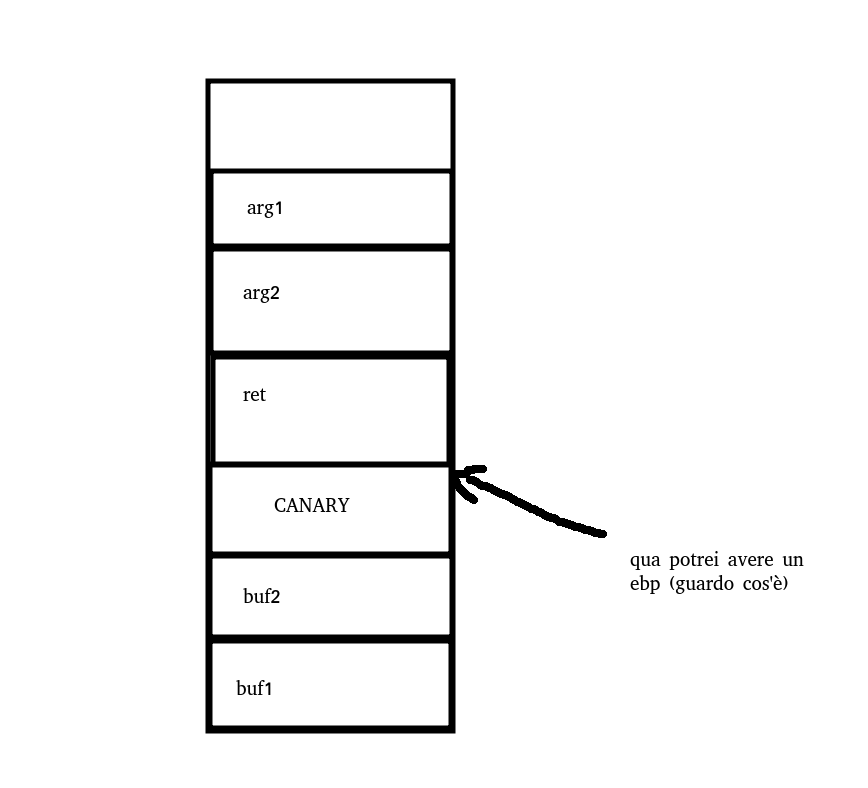
\includegraphics[width=0.4\linewidth]{Immagini/Canary1}
	\caption{Stack con canarino}
\end{figure}

\subsection{DEP Data Execution Prevention}
Vengono resi lo stack e le heap non eseguibili (non dovrebbero contenere codice), e se provo a metterci dello shellcode il sistema operativo lancia un'eccezione.\\
Quindi, come faccio ora a fare l'hackerino?
\subsubsection{Return-to-lib-c}
In memoria ho comunque molto codice. Nelle librerie c che vengono caricate automaticamente è presente \texttt{SYSTEM()}. Quindi, al posto del \texttt{RET} metto l'indirizzo del system, e passo \texttt{"/bin/sh"} come argomento.
\begin{figure}[H]
	\centering
	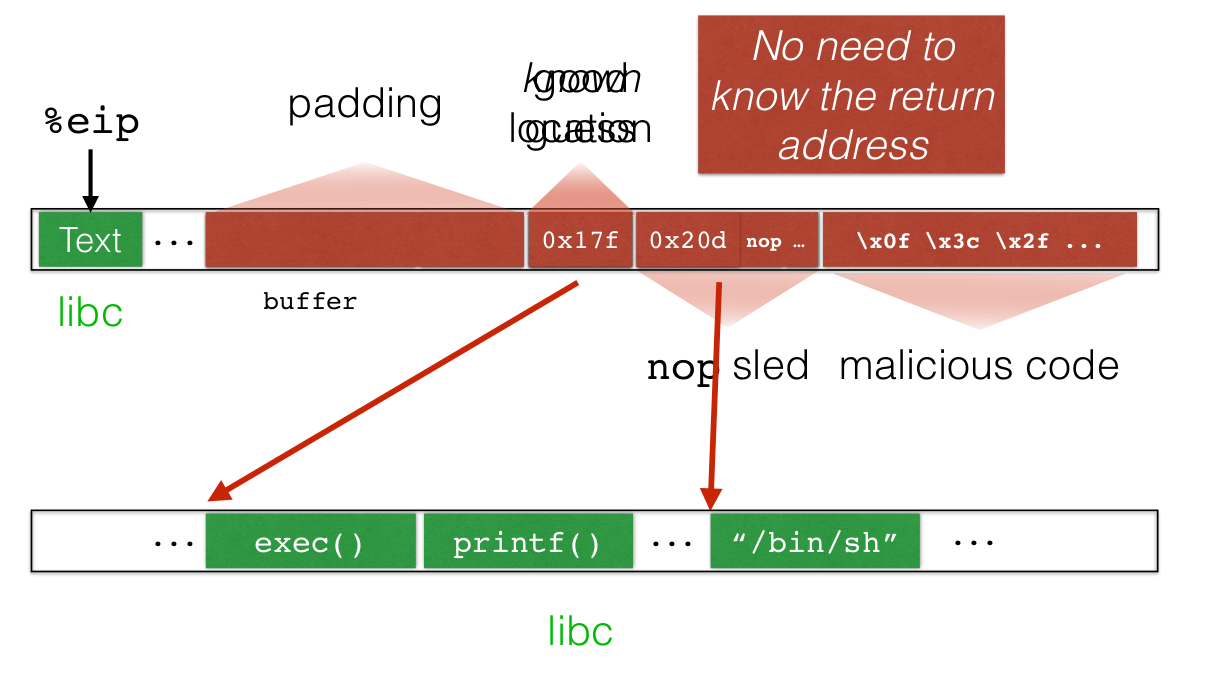
\includegraphics[width=1\linewidth]{Immagini/libc}
	\caption{Return to libc}
\end{figure}


\subsection{Adress space layout randomization}
Ogni volta che ho un programma, carico le zone di memoria (HEAP, TEXT, STACK, BSS) in ordine diverso. Ho alcuni problemi:
\begin{itemize}
\item Shifto solo i blocchi, ms non le posizioni relative all'interno di essi.
\item \E più applicabile alle librerie che al codice del programma vero e proprio.
\item Funziona male con 32 bit, perchè posso fare il brute force dell'indirizzo.
\end{itemize}

\lessonDate{7 Novembre 2019}
\section{Return-oriented Programming (ROP)}
Attacco che usa pezzi di codice già esistenti, detti \textbf{gadget}, che vengono composti in modo \textbf{automatico} per comporre del codice malevolo. Bisogna quindi trovare i gadget e poi concatenarli insieme.\\
Un gadget è un gruppo di istruzioni che termina sempre con un \texttt{ret}. Concateno questi gadget passando ad ogni gadget l'indirizzo del gadget successivo, attraverso le istruzioni \texttt{pop} dello stack. Alla fine, riesco sempre a trovare dei gadget, perchè l'architettura Inter x86 è CISC, ed è piena di istruzioni che possiamo usare, posso saltare in mezzo alle istruzioni, e il codice è self-reparing.\\
Per scrivere il codice malevolo, si usa un cosidetto \textbf{ROP Compiler}. Questo tool si occupa di prendere il codice dell'attacco (scritto in C) e il programma vittima, e mi fornisce il codice assembler da inserire al momento dell'attacco.

\subsection{Blind ROP}
Attacco che ha come vittima un server remoto (linux). Non conosco l'ambiente, e quindi non so dove sono i gadget. Ci sono canarini, randomization ecc. L'idea è quella di farsi dare una copia dell'eseguibile, in modo tale da poter poi costruire  l'exploit.
Condizioni:
\begin{itemize}
\item Macchina a 64 bit
\item ASLR abilitato
\item Canarini abilitati
\end{itemize}

Ad ogni collegamento ad un server, viene creato un thread nel server per gestire la connessione con il client. Questo thread prende le caratteristiche del processo padre, ma in caso di crash viene ricreato \textbf{senza randomizzazione}. L'attacco si svolge così:
\begin{itemize}
\item \textbf{Stack reading:} leggo i canarini e il return address sullo stack.
\item Trovo i gadget che mi permetto di usare la funzione \texttt{write}.
\item Trovo i gadget per trovare tutti gadget per costruire lo shellcode.
\item Ora posso eseguire un rop classico.
\end{itemize}
Quando individuo i gadget, li divido nelle seguenti categorie:
\begin{itemize}
\item \textbf{Crash:} causano il crash del programma
\item \textbf{Infinite Loop:} gadget che possono essere chiamati indefinitamente. Sono particolarmente interessato a quelli che eseguono operazioni sullo stack.
\end{itemize}


\end{document}
